\documentclass[14pt]{extbook}
\usepackage{multicol, enumerate, enumitem, hyperref, color, soul, setspace, parskip, fancyhdr} %General Packages
\usepackage{amssymb, amsthm, amsmath, latexsym, units, mathtools} %Math Packages
\everymath{\displaystyle} %All math in Display Style
% Packages with additional options
\usepackage[headsep=0.5cm,headheight=12pt, left=1 in,right= 1 in,top= 1 in,bottom= 1 in]{geometry}
\usepackage[usenames,dvipsnames]{xcolor}
\usepackage{dashrule}  % Package to use the command below to create lines between items
\newcommand{\litem}[1]{\item#1\hspace*{-1cm}\rule{\textwidth}{0.4pt}}
\pagestyle{fancy}
\lhead{Progress Quiz 6}
\chead{}
\rhead{Version A}
\lfoot{1430-1829}
\cfoot{}
\rfoot{test}
\begin{document}

\begin{enumerate}
\litem{
Construct the lowest-degree polynomial given the zeros below. Then, choose the intervals that contain the coefficients of the polynomial in the form $x^3+bx^2+cx+d$.\[ 5 + 3 i \text{ and } 3 \]\begin{enumerate}[label=\Alph*.]
\item \( b \in [10, 18], c \in [62.11, 64.76], \text{ and } d \in [101, 106.3] \)
\item \( b \in [-21, -5], c \in [62.11, 64.76], \text{ and } d \in [-105.1, -100.1] \)
\item \( b \in [1, 3], c \in [-8.79, -7.83], \text{ and } d \in [11.8, 17] \)
\item \( b \in [1, 3], c \in [-7.39, -4.76], \text{ and } d \in [5.2, 9.5] \)
\item \( \text{None of the above.} \)

\end{enumerate} }
\litem{
Describe the end behavior of the polynomial below.\[ f(x) = 8(x - 6)^{4}(x + 6)^{9}(x + 9)^{4}(x - 9)^{5} \]\begin{enumerate}[label=\Alph*.]
\begin{multicols}{2}\item 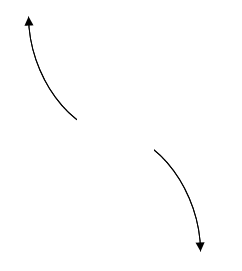
\includegraphics[width = 0.3\textwidth]{../Figures/polyEndBehaviorCopyAA.png}\item 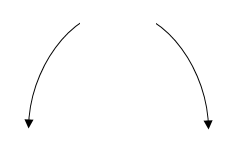
\includegraphics[width = 0.3\textwidth]{../Figures/polyEndBehaviorCopyBA.png}\item 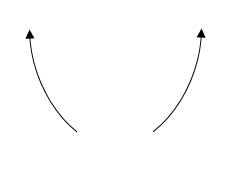
\includegraphics[width = 0.3\textwidth]{../Figures/polyEndBehaviorCopyCA.png}\item 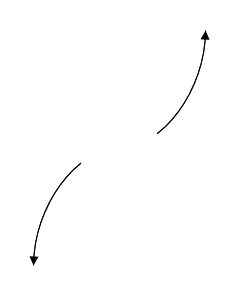
\includegraphics[width = 0.3\textwidth]{../Figures/polyEndBehaviorCopyDA.png}\end{multicols}\item None of the above.
\end{enumerate} }
\litem{
Describe the zero behavior of the zero $x = 7$ of the polynomial below.\[ f(x) = 9(x + 7)^{8}(x - 7)^{11}(x - 3)^{7}(x + 3)^{10} \]\begin{enumerate}[label=\Alph*.]
\begin{multicols}{2}\item 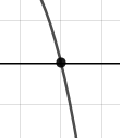
\includegraphics[width = 0.3\textwidth]{../Figures/polyZeroBehaviorAA.png}\item 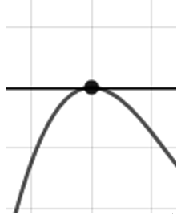
\includegraphics[width = 0.3\textwidth]{../Figures/polyZeroBehaviorBA.png}\item 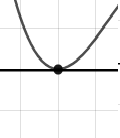
\includegraphics[width = 0.3\textwidth]{../Figures/polyZeroBehaviorCA.png}\item 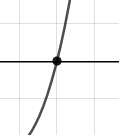
\includegraphics[width = 0.3\textwidth]{../Figures/polyZeroBehaviorDA.png}\end{multicols}\item None of the above.
\end{enumerate} }
\litem{
Construct the lowest-degree polynomial given the zeros below. Then, choose the intervals that contain the coefficients of the polynomial in the form $ax^3+bx^2+cx+d$.\[ \frac{-5}{3}, -3, \text{ and } \frac{5}{4} \]\begin{enumerate}[label=\Alph*.]
\item \( a \in [12, 15], b \in [-43, -40], c \in [-16, -2], \text{ and } d \in [71, 81] \)
\item \( a \in [12, 15], b \in [37, 49], c \in [-16, -2], \text{ and } d \in [71, 81] \)
\item \( a \in [12, 15], b \in [-2, 3], c \in [-84, -79], \text{ and } d \in [71, 81] \)
\item \( a \in [12, 15], b \in [37, 49], c \in [-16, -2], \text{ and } d \in [-78, -73] \)
\item \( a \in [12, 15], b \in [-85, -66], c \in [126, 135], \text{ and } d \in [-78, -73] \)

\end{enumerate} }
\litem{
Construct the lowest-degree polynomial given the zeros below. Then, choose the intervals that contain the coefficients of the polynomial in the form $ax^3+bx^2+cx+d$.\[ \frac{-6}{5}, \frac{-4}{3}, \text{ and } -3 \]\begin{enumerate}[label=\Alph*.]
\item \( a \in [13, 21], b \in [76, 90], c \in [133, 140], \text{ and } d \in [-75, -70] \)
\item \( a \in [13, 21], b \in [42, 53], c \in [-19, -16], \text{ and } d \in [-75, -70] \)
\item \( a \in [13, 21], b \in [3, 8], c \in [-91, -85], \text{ and } d \in [66, 76] \)
\item \( a \in [13, 21], b \in [-84, -78], c \in [133, 140], \text{ and } d \in [-75, -70] \)
\item \( a \in [13, 21], b \in [76, 90], c \in [133, 140], \text{ and } d \in [66, 76] \)

\end{enumerate} }
\litem{
Which of the following equations \textit{could} be of the graph presented below?
\begin{center}
    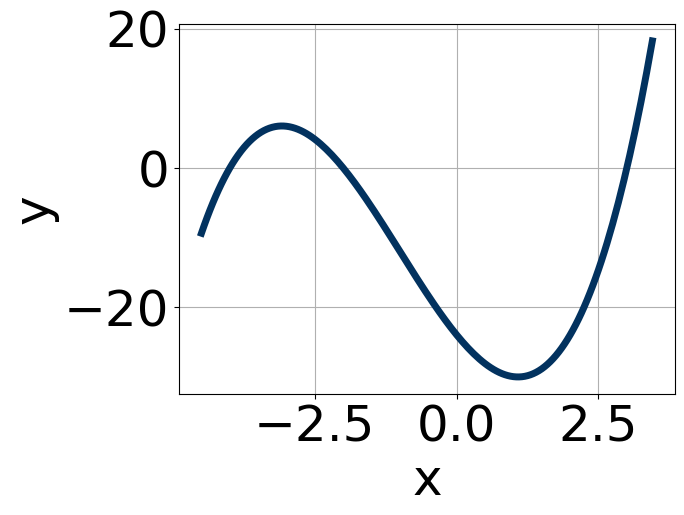
\includegraphics[width=0.5\textwidth]{../Figures/polyGraphToFunctionCopyA.png}
\end{center}
\begin{enumerate}[label=\Alph*.]
\item \( -11(x + 4)^{7} (x - 1)^{7} (x + 3)^{11} \)
\item \( -3(x + 4)^{8} (x - 1)^{11} (x + 3)^{11} \)
\item \( 18(x + 4)^{8} (x - 1)^{7} (x + 3)^{5} \)
\item \( 6(x + 4)^{4} (x - 1)^{10} (x + 3)^{5} \)
\item \( 20(x + 4)^{9} (x - 1)^{11} (x + 3)^{7} \)

\end{enumerate} }
\litem{
Which of the following equations \textit{could} be of the graph presented below?
\begin{center}
    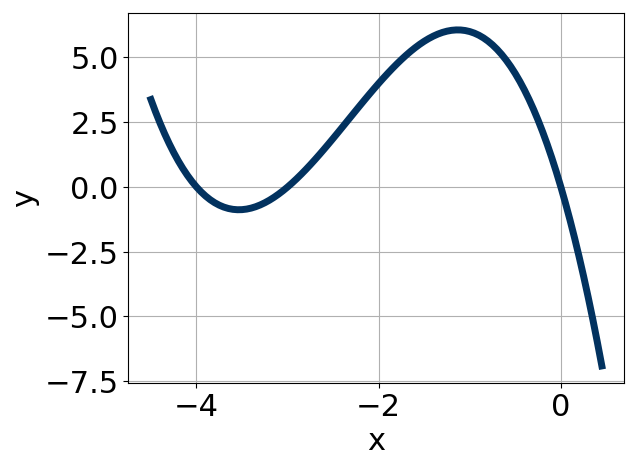
\includegraphics[width=0.5\textwidth]{../Figures/polyGraphToFunctionA.png}
\end{center}
\begin{enumerate}[label=\Alph*.]
\item \( -5(x + 4)^{10} (x - 3)^{11} (x + 2)^{7} \)
\item \( -11(x + 4)^{6} (x - 3)^{10} (x + 2)^{5} \)
\item \( 9(x + 4)^{6} (x - 3)^{10} (x + 2)^{11} \)
\item \( -19(x + 4)^{4} (x - 3)^{9} (x + 2)^{6} \)
\item \( 19(x + 4)^{4} (x - 3)^{8} (x + 2)^{4} \)

\end{enumerate} }
\litem{
Describe the zero behavior of the zero $x = -7$ of the polynomial below.\[ f(x) = -8(x - 7)^{8}(x + 7)^{13}(x - 9)^{4}(x + 9)^{7} \]\begin{enumerate}[label=\Alph*.]
\begin{multicols}{2}\item 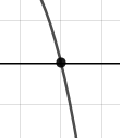
\includegraphics[width = 0.3\textwidth]{../Figures/polyZeroBehaviorCopyAA.png}\item 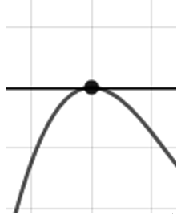
\includegraphics[width = 0.3\textwidth]{../Figures/polyZeroBehaviorCopyBA.png}\item 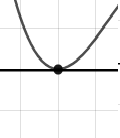
\includegraphics[width = 0.3\textwidth]{../Figures/polyZeroBehaviorCopyCA.png}\item 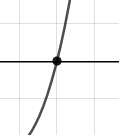
\includegraphics[width = 0.3\textwidth]{../Figures/polyZeroBehaviorCopyDA.png}\end{multicols}\item None of the above.
\end{enumerate} }
\litem{
Construct the lowest-degree polynomial given the zeros below. Then, choose the intervals that contain the coefficients of the polynomial in the form $x^3+bx^2+cx+d$.\[ -5 + 3 i \text{ and } 1 \]\begin{enumerate}[label=\Alph*.]
\item \( b \in [4, 10], c \in [22, 26], \text{ and } d \in [-38, -33] \)
\item \( b \in [-16, -7], c \in [22, 26], \text{ and } d \in [27, 36] \)
\item \( b \in [-4, 5], c \in [1, 6], \text{ and } d \in [-12, -3] \)
\item \( b \in [-4, 5], c \in [-4, 0], \text{ and } d \in [2, 4] \)
\item \( \text{None of the above.} \)

\end{enumerate} }
\litem{
Describe the end behavior of the polynomial below.\[ f(x) = -4(x + 4)^{3}(x - 4)^{6}(x - 5)^{2}(x + 5)^{3} \]\begin{enumerate}[label=\Alph*.]
\begin{multicols}{2}\item 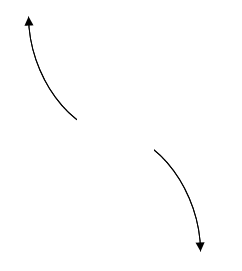
\includegraphics[width = 0.3\textwidth]{../Figures/polyEndBehaviorAA.png}\item 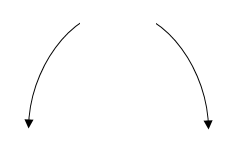
\includegraphics[width = 0.3\textwidth]{../Figures/polyEndBehaviorBA.png}\item 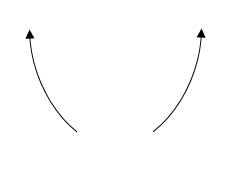
\includegraphics[width = 0.3\textwidth]{../Figures/polyEndBehaviorCA.png}\item 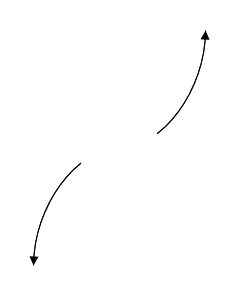
\includegraphics[width = 0.3\textwidth]{../Figures/polyEndBehaviorDA.png}\end{multicols}\item None of the above.
\end{enumerate} }
\end{enumerate}

\end{document}